\documentclass[a4paper, 11pt]{article}

% DEFINIËREN CODERING
\usepackage[utf8]{inputenc}

% DEFINIËREN BLAD
\usepackage[
top=20mm,
bottom=20mm,
left=20mm,
right=20mm,
heightrounded,
]{geometry}
\usepackage{lastpage}
\usepackage{fancyhdr}
%\pagestyle{fancy}
\fancyhead[L]{}
\fancyhead[C]{}
\fancyhead[R]{}
\fancyfoot[L]{}
\fancyfoot[C]{\thepage}
\fancyfoot[R]{}
\renewcommand{\headrulewidth}{0pt}
\renewcommand{\footrulewidth}{.4pt}
\setlength{\headheight}{13.6pt}
\setlength{\parindent}{1cm}

% MEDIA
% Tabellen
\usepackage{array}
\newcolumntype{L}[1]{>{\raggedright\let\newline\\\arraybackslash\hspace{0pt}}m{#1}}
\newcolumntype{C}[1]{>{\centering\let\newline\\\arraybackslash\hspace{0pt}}m{#1}}
\newcolumntype{R}[1]{<{\raggedleft\let\newline\\\arraybackslash\hspace{0pt}}m{#1}}
\usepackage{stackengine}
\newcommand\xrowht[2][0]{\addstackgap[.5\dimexpr#2\relax]{\vphantom{#1}}}
\usepackage{tabularx}
\usepackage{multirow}
\usepackage{hhline}
\usepackage{float}
% Afbeeldingen
\usepackage{graphicx}
% Figuren
\usepackage{tikz}

% WISKUNDE
% Basis
\usepackage{amsmath}
\usepackage{amssymb}
\usepackage{amsthm}
% Aanpassing
\usepackage{dsfont}   % Voor de natuurlijke, gehele, rationele, reële, complexe getallen => ``$\mathfb{}$''
\usepackage{mathdots} % Voor betere puntjes
\usepackage{esvect}   % Voor betere vectorpijltjes => ``$\vv{}$''
\usepackage{textcomp} % Nodig om gensymb correct te laten werken
\usepackage{gensymb}  % Invoegen van enkele symbolen => ``\degree ; \celcius ; \perthousand ; \ohm ; \micro''
\usepackage{cancel}   % Voor het beter doorstrepen van zaken => ``\cancel ; \bcancel ; \xcancel''
\usepackage{esint}    % Meervoudige kringintegralen
\usepackage{hyperref}

\newcommand{\naar}{\,$\rightarrow$\,}
\newcommand{\ppp}{\ldots}
\renewcommand{\empty}{$\varnothing$}
\newcommand{\of}{$\cup$}
\newcommand{\<}{\scriptsize\textless\normalsize}
\renewcommand{\>}{\scriptsize\textgreater\normalsize}

% Voorblad
\title{Programmeerproject 2: Besturingssysteem Modeltreinen\\ Handleiding voor Eindgebruikers}
\author{Jonas Br\"ull, 0587194\\ Jonas.Simon.E.Brull@vub.be\\}
\date{Academiejaar 2024-2025\\Vrije Universiteit Brussel}


% BEGIN DOCUMENT ==================================================================================
\begin{document}

\pagenumbering{gobble}
\maketitle
\newpage

\pagenumbering{gobble}
\tableofcontents
\newpage

\pagestyle{fancy}
\setcounter{page}{1}
\pagenumbering{arabic}

% =================================================================================================
\section{Introductie} % ===========================================================================
Dit document beschrijft de handleiding van mijn implementatie van een Modeltrein Software Toepassing in de programmeertaal Racket. Het is deel van het opleidingsonderdeel ``Programmeerproject 2''.


% =================================================================================================
\section{Nodige Software en Bestanden} % =======================================================================
Alle benodigde bestanden zijn gebundeld in het zip-bestand ``besturingssysteem-modeltreinen.zip'' of te vinden op de GitHub repository van het project. De applicatie is geschreven in de programmeertaal Racket, en kan worden uitgevoerd met DrRacket.\\\\
De applicatie is afhankelijk van de volgende Racket packages:
\begin{itemize}
  \item \textbf{racket/gui}:  Voor de gui elementen.
  \item \textbf{racket/date}: Voor het werken met datum \& tijd tijdens het loggen van gebeurtenissen. 
  \item \textbf{racket/exn}:  Voor het afhandelen van uitzonderingen.
  \item \textbf{try-catch}:   Voor het afhandelen van fouten tijdens het opstarten. 
\end{itemize}
Buiten try-catch, zijn deze packages standaard geïnstalleerd in DrRacket. DrRacket zal normaal gezien zelf voorstellen om try-catch te installeren.

\subsection{Installatie DrRacket} %----------------------------------------------------------------
DrRacket is te vinden op de website: \url{https://racket-lang.org/} onder "Download". De standaardwaarden bij het installeren van DrRacket zijn voldoende voor dit project.

\subsection{Opstarten} %---------------------------------------------------------------------------
Het opstarten van de applicaties gebeurt via het openen van volgende bestanden in DrRacket:
\begin{itemize}
  \item \textbf{Infrabel}: INFRABEL.rkt
  \item \textbf{Providers}: NMBS.rkt, andere geconfigureerde providers.
\end{itemize}
De andere bestanden bevatten de applicatie logica en hoeven niet geopend te worden.\\
\begin{figure}[h]
	\begin{center}
		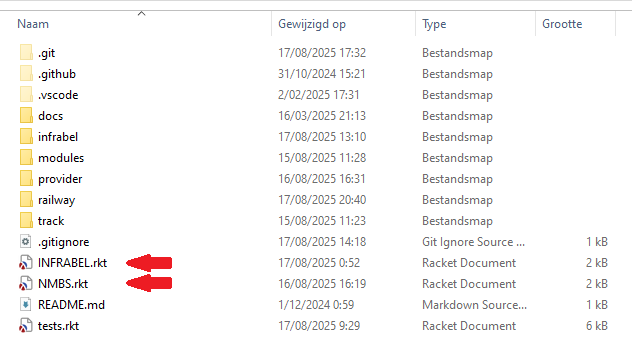
\includegraphics[scale=.60]{Bestanden/besturingssysteem-modeltreinen-tldir.png}
		\caption{Top Level Directory van het project}
	\end{center}
\end{figure}

\newpage
% =================================================================================================
\section{Infrabel} % ==============================================================================
\subsection{Opstarten} %---------------------------------------------------------------------------
Om de Infrabel applicatie te starten, moet het bestand INFRABEL.rkt geopend worden in DrRacket. Hierna moet je op het groene pijltje (start-knop) rechts-boven drukken. Het programma zal opstarten en de "Infrabel startup manager" zal openen.
\begin{figure}[h]
	\begin{center}
		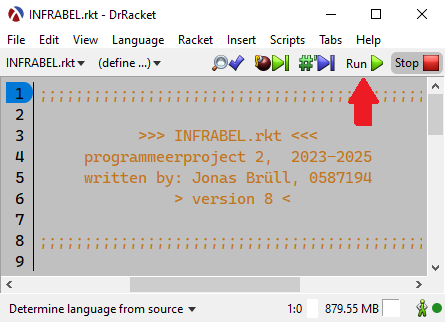
\includegraphics[scale=.5]{Bestanden/infrabel-rkt.png}
		\caption{Opstarten van Infrabel via DrRacket}
	\end{center}
\end{figure}
\\In de Startup Manager kan je de instellingen aanpassen:
\begin{itemize}
  \item \textbf{Railway Architecture}: Infrabel kan verbinding maken met zowel simulators, als hardware opstellingen. Hier kun je aanpassen met welke opstelling je wilt werken. Let op: voor hardware, moet je eerst verbinding maken met de Z21 Command \& Control centrale van de harware.
  \item \textbf{Simulator version}: Hier kan je de versie van de simulator kiezen. Deze optie wordt uitgeschakeld als je voor hardware koos als architecture.
  \item \textbf{Hostname}: Standaard zal de infrabel server op localhost draaien, maar als je Infrabel op een Raspberry Pi wilt draaien, kun je hier het IP-address ingeven.
  \item \textbf{Port}: Hier kan je de poort van de Infrabel server kiezen. Standaard poort is 2020.
  \item \textbf{Start with Control Panel}: Indien je een Controle Paneel (GUI) wenst om Infrabel aan te sturen (bijvoorbeeld om fouten op te lossen), kun je deze optie aanvinken.
\end{itemize}
De standaard instellingen zijn voldoende om Infrabel te laten werken en gebruik je best ook als je de software voor de eerste keer gebruikt.\\
Na het aanpassen van de instellingen, kun je op de knop "Start" drukken. Infrabel zal nu opstarten en verbinding maken met de simulator of hardware.\\
Moest er een fout optreden tijdens het opstarten, kun je deze terugvinden in het "Log Paneel", naast de instellingen. Hier zal ook de log van de opstart verschijnen.\\
\begin{figure}[h]
	\begin{center}
		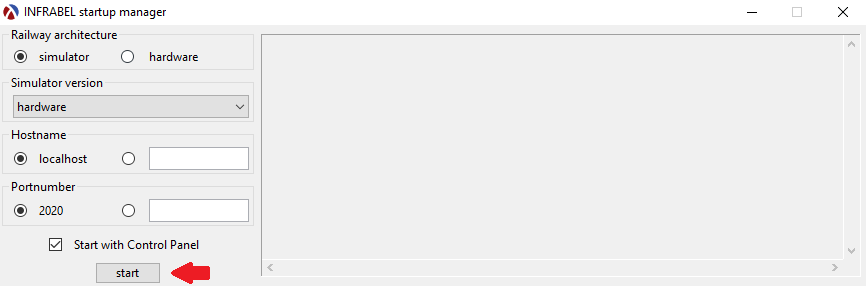
\includegraphics[scale=.5]{Bestanden/infrabel-startup-rkt.png}
		\caption{Opstarten van Infrabel via de Startup Manager}
	\end{center}
\end{figure}

\newpage

\subsection{Controle Paneel} %-------------------------------------------------------------------
\begin{figure}[h]
	\begin{center}
		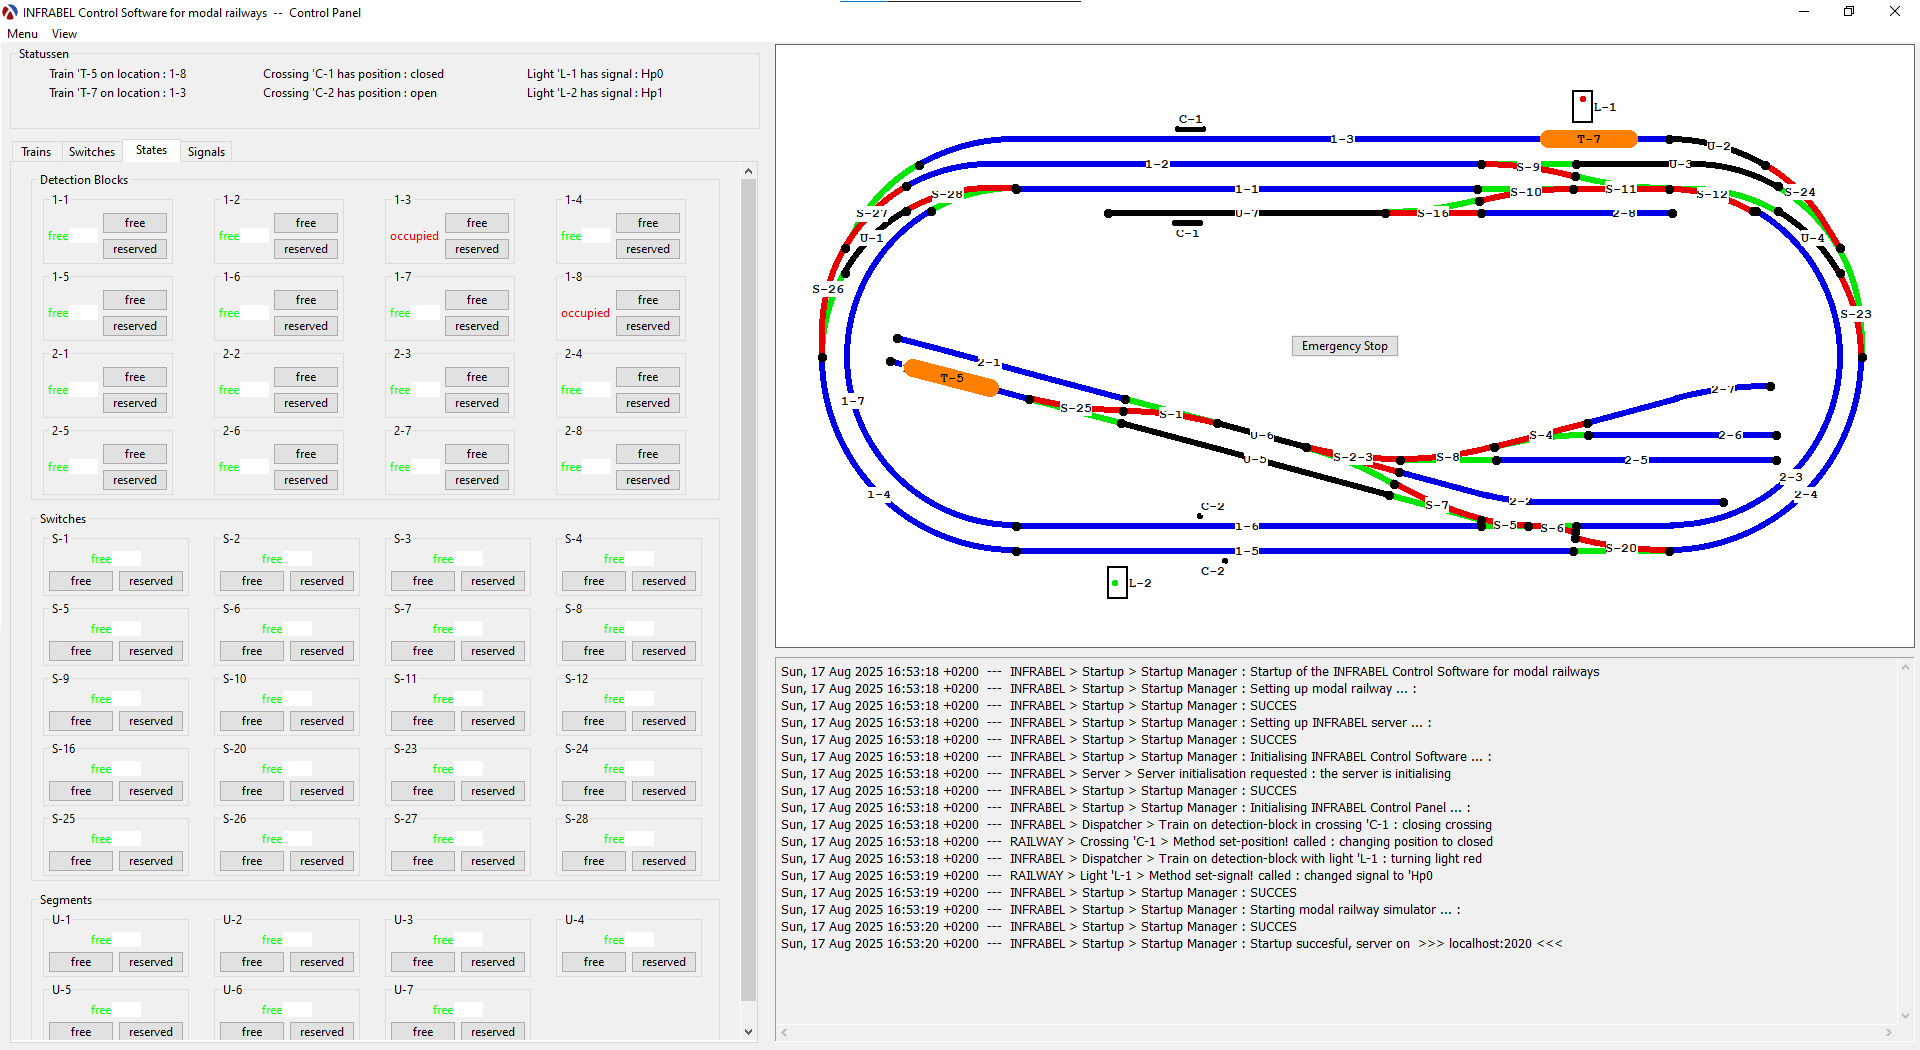
\includegraphics[scale=.35]{Bestanden/infrabel-gui-rkt.png}
		\caption{Infrabel controle paneel}
	\end{center}
\end{figure}

Het controle paneel bestaat uit 3 elementen: de embedded simulator (indien de hardware bestuurd wordt, wordt deze niet getoond), een log-paneel waar de logs in read time getoond worden en het besturingspaneel, met daarboven de statussen van enkele belangrijke elementen.\\
Het besturingspaneel bestaat uit verschillende tabbladen:
\begin{itemize}
  \item \textbf{Treinen}: Hier kunnen treinen handmatig bestuurd worden. (zie verder)
  \item \textbf{Wissels}: Hier kunnen wissels handmatig bestuurd worden. Elke wissel wordt voorgesteld in zijn eigen elementje en heeft twee knoppen, een knop om de wissel in de "linkse" stand te plaatsen en een knop om de wissel in de "rechtse" stand te plaatsen, altijd bekeken vanuit de kan met 1 uitgang naar de kant met 2 uitgangen.
  \item \textbf{Statussen}: Elk element van de railway waarop de trein kan rijden, heeft een status. Hier kunnen deze statussen bekeken en handmatig aangepast worden. Zoals bij de wissels worden de spoorelementen hier voorgesteld met twee knoppen, een om het element "vrij te maken" en een om het element te "reserveren".
  \item \textbf{Signalen}: Hier kunnen de overwegen en lichten handmatig bestuurd worden door middel van de knoppen, die dit signaal dan doorgeven.
\end{itemize}
De elementen in deze tabbladen worden automatisch geupdatet wanneer de elementen in de railway veranderen. Ook heeft infrabel de mogelijkheid om overwegen, lichten, wissels en treinen aan te sturen. Zo zullen bijvoorbeeld de lichten automatisch op rood springen en de slagbomen automatisch sluiten, indien er een trein gedetecteerd wordt.\\\\
Het controle paneel is vooral bedoeld om testen uit te voeren en om fouten op te lossen, op en binnen infrabel zelf, zonder dat er providers of TCP verbindingen extra plaatsen kunnen toevoegen waar er zicht fouten kunnen voordoen. 

\newpage
\subsection{Treinen} %-----------------------------------------------------------------------
De treinen kunnen handmatig bestuurd worden vanuit het tabblad "Trains". Hier worden
\begin{figure}[h]
	\begin{center}
		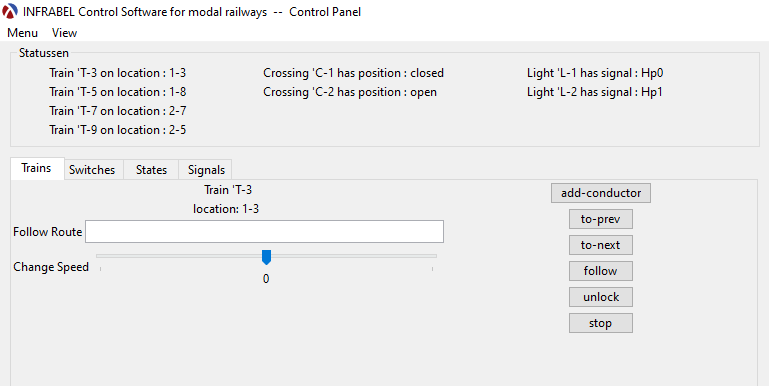
\includegraphics[scale=.75]{Bestanden/infrabel-train.png}
		\caption{Infrabel controle paneel}
	\end{center}
\end{figure}

Voor een trein om automatisch te kunnen rijden, moet deze een conducteur hebben. Als je op de knop "add-conductor" drukt, wordt er een conducteur aan de trein toegevoegd.
Enkel als de trein een conducteur heeft, kunnen de knoppen "to-prev" en "to-next" gebruikt worden. Deze zullen de trein naar het vorige/volgende detectieblok laten rijden.
Via de knop "follow" zal de trein de route opgegeven in het invoerveld "follow route" (TODO: implementeer follow-route) volgen.
Via de knop "unlock" kan de trein ontgrendeld worden en kan deze terug aanstuurbaar worden door middel van de gui. Treinen worden "gelocked" door het programma als ze een pad volgen.
De knop "stop" zal de trein doen stoppen. De snelheid van de trein kan aangepast worden via de "change-speed" schuifbalk.

\newpage
% =================================================================================================
\section{Providers} % =============================================================================
\subsection{Opstarten} %---------------------------------------------------------------------------
Om een provider applicatie te starten, moet het bestand NMBS.rkt (of andere geconfigureerde provider) geopend worden in DrRacket. Hierna moet je op het groene pijltje (start-knop) rechts-boven drukken. Het programma zal opstarten en een provider "startup manager" zal openen.\\

\begin{figure}[h]
	\begin{center}
		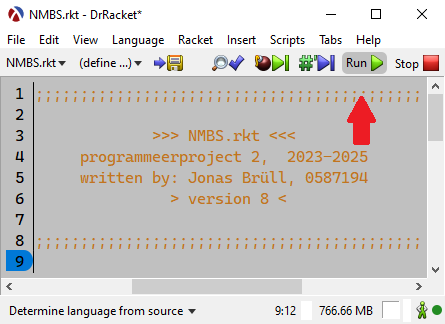
\includegraphics[scale=.5]{Bestanden/provider.png}
		\caption{Opstarten van Provider via DrRacket}
	\end{center}
\end{figure}

In de startup manager kun je de hostname en poortnummer aanpassen, indien de infrabel server niet op de standaard instellingen draait.

\begin{figure}[h]
	\begin{center}
		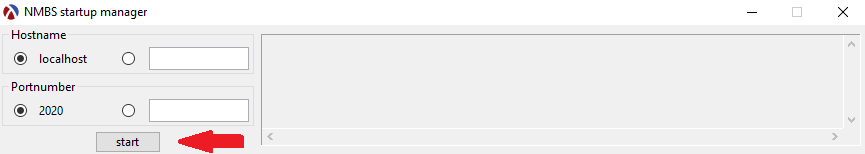
\includegraphics[scale=.5]{Bestanden/provider-startup-rkt.png}
		\caption{Opstarten van Provider via de Startup Manager}
	\end{center}
\end{figure}

% =================================================================================================
\label{lastpage}
\end{document}
